\documentclass[t,handout]{beamer}
\usepackage{verbatim}
\usepackage{xcolor}
\usepackage{multirow}
\usepackage{amssymb}
\usepackage{tikz}
\usepackage{hyperref}
\usetikzlibrary{positioning,fit}
%\usepackage{enumitem}
\usetheme{Warsaw}
\setbeamertemplate{navigation symbols}{}
\newcommand{\blue}[1]{{\color{blue} #1}}
\newcommand{\red}[1]{{\color{red} #1}}
\newcommand{\grn}[1]{{\color{green} #1}}
\newcommand{\bluRed}[2]{{\color{blue} #1}{\color{red} #2}}
\newcommand{\qtns}[0]{\begin{center} Questions? \end{center}}
\newcommand{\nl}[1]{\vspace{#1 em}}
\newcommand{\cntrImg}[2]{\begin{center}\includegraphics[scale=#2]{#1}\end{center}}
\newcommand{\defn}[1]{{\bf #1}}
\let\emptyset\varnothing
\newcommand{\SampS}[0]{$\mathcal{S}$}

\title{Math 3070, Applied Statistics}

\begin{document}
\begin{frame}[c]
    \begin{beamercolorbox}[rounded=true,wd=\textwidth,center]{title}
        \usebeamerfont{title}\inserttitle
    \end{beamercolorbox}
    \begin{center}
        Section 1\\
        \nl{0.5}
        October 4, 2019
    \end{center}
\end{frame}
\begin{frame}[c]{Lecture Outline, 10/4}
    Section 5.1
    \begin{itemize}
        \item Joint Probability Density Functions
        \item Marginal PDFs
        \item Independence
        \item Conditional PDFs
    \end{itemize}
\end{frame}
\begin{frame}[c]{Joint Probability Density}
    \begin{block}{}
        Random variables $X$ and $Y$ are said to have a \textbf{joint probability density} (joint pdf) $f(x,y)$ if
        \begin{align*}
            P(a \leq X \leq b, c \leq Y \leq d) & = P(a \leq X \leq b \cap c \leq Y \leq d) \\
                                                & = \int_a^b\int_c^d f(x,y)\ dy\ dx         \\
        \end{align*}
        for all real constants $a\leq b$ and $c\leq d$.\\
        Need $f(x,y)\geq 0$ and $\int_{-\infty}^\infty\int_{-\infty}^\infty f(x,y)\ dy\ dx=1$
    \end{block}
\end{frame}

\begin{frame}{Example, Check PDF}
    \begin{block}{}
        A bank operates a drive-up facility and a walk-up window. On a random day, let $X$ be the proportion of time the drive-up facility is in use, and let $Y$ be the proportion of time the walk-up window is in use. Check that a valid joint pdf for $X$ and $Y$ is given by
        $$f(x,y)=\begin{cases}\frac65(x+y^2), & 0\leq x \leq 1, 0\leq y\leq 1 \\ 0, & \text{otherwise}\end{cases}$$
    \end{block}
    \uncover<1->{$f(x,y)\geq 0$}
    \begin{align*}
        \uncover<2->{\int_{-\infty}^\infty\int_{-\infty}^\infty f(x,y)\ dy\ dx & = \int_0^1\int_0^1 \frac65(x+y^2)\ dy\ dx}                                                    \\
        \uncover<3->{                                             & =\frac65 \int_0^1 \left(xy+\frac{y^3}3\right)\Big\vert_{y=0}^1\ dx \\}
        \uncover<4->{                                             & = \frac65\int_0^1 \left(x+ \frac13\right)\ dx}
        \uncover<5->{= \frac65\left(\frac12+\frac13\right) }
        \uncover<6->{= 1}
    \end{align*}
\end{frame}

\begin{frame}{Marginal Probability Density Function}
    \begin{block}{}
        Let $X$ and $Y$ be random variables with joint pdf $f(x,y)$. The \textbf{marginal probability density function} (marginal pdf) of $X=x$ is defined as
        $$f_X(x) = \int_{-\infty}^\infty f(x,y)\ dy$$
        Similarly, the marginal pdf of $Y$ is
        $$f_Y(y) = \int_{-\infty}^\infty f(x,y)\ dx$$
    \end{block}

    \pause Note: $f_X$ is simply the pdf of $X$ considered as a random variable on its own. Same as $f_X (x)$ for PDFs.
\end{frame}

\begin{frame}{Example, Marginal PDF}
    \begin{block}{}
        In the bank example, the joint pdf of two random variables $X$ and $Y$ was given by
        $$f(x,y)=\begin{cases}\frac65(x+y^2), & 0\leq x \leq 1, 0\leq y\leq 1 \\ 0, & \text{otherwise}\end{cases}$$
        Find the marginal pdf of $X$.
    \end{block}
    \pause \vspace{-.2cm}\begin{align*}
        f_X(x)        & = \int_{-\infty}^\infty f(x,y)\ dy                      \\
        \uncover<3->{ & = \int_0^1 \frac65(x+y^2)\ dy \\}
        \uncover<4->{ & = \frac65\left(xy+\frac{y^3}3\right)\Big\vert_{y=0}^1}
        \uncover<5->{= \frac65\left(x+\frac13\right)}
    \end{align*}
\end{frame}

\begin{frame}[c]{Independence}
    \begin{block}{}
        $X$ and $Y$ are \textbf{independent} continuous random variables if their joint pdf is the product of the marginal pdfs:
        $$f(x,y) = f_X(x)f_Y(y)$$
        Their events are also independent, $P(a<X<b \cap c<Y<d) = P(a<X<b)P(c<Y<d)$.
    \end{block}
\end{frame}

\begin{frame}{Example, Independence}
    \begin{block}{}
        A system has two components; assuming their lifetimes $X$ and $Y$ are independent exponential random variables with $E(X)=10$ and $E(Y)=20$, what is the probability that the first component outlasts the second?
    \end{block}

    \pause\vspace{-.2cm}
    \begin{tabular}{p{7.2cm}p{4cm}}
        \vspace{0cm}$\begin{aligned}[t]
                P(X\geq Y)    & = \int_0^\infty\int_y^\infty f(x,y)\ dx\ dy                                                              \\
                \uncover<3->{ & = \int_0^\infty\int_y^\infty \frac1{200}e^{-\frac{x}{10}-\frac{y}{20}}\ dx\ dy \\}
                \uncover<4->{ & = \frac1{200}\int_0^\infty e^{-y/20}\int_y^\infty e^{-x/10}\ dx\ dy \\}
                \uncover<5->{ & = \frac1{200}\int_0^\infty e^{-y/20}\cdot 10e^{-y/10}\ dy \\}
                \uncover<6->{ & = \frac1{20}\int_0^\infty e^{-\frac3{20}y}\ dy }
                \uncover<7->{= \frac1{20}\cdot \frac{20}3 }
                \uncover<8->{= \frac13}
            \end{aligned}$
         & \vspace{-.2cm}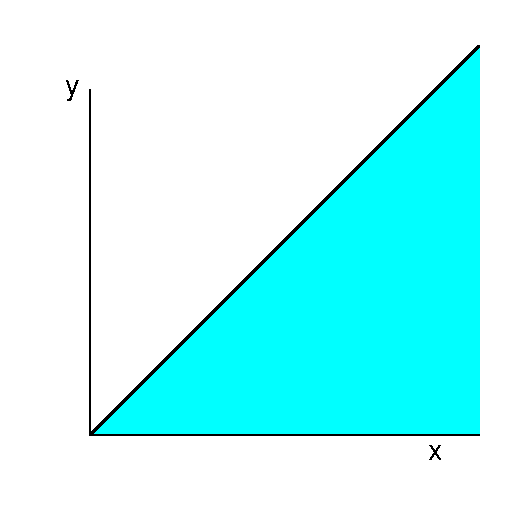
\includegraphics[scale=.4]{ch5_xy.pdf}
    \end{tabular}
\end{frame}

\begin{frame}{Conditional Probability Density Function}
\begin{block}{}
Let $X$ and $Y$ be random variables with joint pdf $f(x,y)$. The \textbf{conditional probability density function} of $Y$ given $X$ is
$$f_{Y\mid X}(y\mid x) = \frac{f(x,y)}{f_X(x)}$$
\end{block}
\pause If $X$ and $Y$ are independent, then the conditional pdf of $Y$ given $X$ is simply the marginal pdf of $Y$:
$$f_{Y\mid X}(y\mid x) = \frac{f(x,y)}{f_X(x)} = \frac{f_X(x)f_Y(y)}{f_X(x)} = f_Y(y)$$
$$ P(a<Y<b|X=x) = \int_{a}^b f_{Y|X}(y|x)dy $$
\pause Note: The event $X=x$ has zero probability. Typically, this is used when one value is already measured. Note, this would be a different calculation for events involving two random varaibles.
\end{frame}

\begin{frame}{Example, Conditional Probability Density Function}
    Recall the bank example. $X$ is the proportion of time the drive-up facility is in use and $Y$ is the proportion of time the walk-up window is in use. They have the following joint PDF,
$$f(x,y)=\begin{cases}\frac65(x+y^2), & 0\leq x \leq 1, 0\leq y\leq 1 \\ 0, & \text{otherwise}\end{cases}$$
    Given that drive-up facility is always in use, what is the probability that the walk-up facility is in use less than half the time?\\
    \uncover<1->{We are conditioning on the event that $X=1$.\\} 
    \uncover<2->{We can use the marginal from the previous example. $$f_X(x) = \frac{6}{5}\bigg(x + \frac{1}{3}\bigg)$$}
    \uncover<3->{$$f_{Y|X}(Y|1) = \frac{f(1,y)}{f_X(1)} = \frac{\frac{6}{5}(1+y^2)}{\frac{6}{5}(1+\frac{1}{3})} = \frac{1+y^2}{1+\frac{1}{3}} = \frac{3}{4} (1+y^2) $$}
    \vfill
\end{frame}

\begin{frame}{Example, Conditional Probability Density Function}
$$f_{Y|X}(y|1)=\begin{cases}
    \frac{3}{4} (1+y^2), & 0\leq y\leq 1 \\ 
0, & \text{otherwise}\end{cases}$$

\begin{align*}
    \uncover<1->{P\bigg(Y<\frac{1}{2}\bigg|X=1\bigg) } & \uncover<2->{=\int^{\frac{1}{2}}_{-\infty} f_{Y|X}(y|1) dy} \\
    & \uncover<3->{=\int^{\frac{1}{2}}_0 \frac{3}{4} (1+y^2) dy} \\
    & \uncover<4->{= \frac{3}{4} \bigg[ y+\frac{y^3}{3} \bigg|_{y=0}^{1/2} \bigg]} \\
    & \uncover<5->{= \frac{3}{4} \bigg[ \frac{1}{2}+\frac{1}{24} \bigg] \approx 0.40625} \\
\end{align*}
    \vfill
\end{frame}

\begin{frame}{Non-Example, Conditional Probability Density Function}
    Recall the bank example. $X$ is the proportion of time the drive-up facility is in use and $Y$ is the proportion of time the walk-up window is in use. They have the following joint PDF,
$$f(x,y)=\begin{cases}\frac65(x+y^2), & 0\leq x \leq 1, 0\leq y\leq 1 \\ 0, & \text{otherwise}\end{cases}$$
    Given that drive-up facility in use less than half the time, what is the probability that the walk-up facility is in use less than half the time?\\
    \vfill
\end{frame}

\begin{frame}{Non-Example, Conditional Probability Density Function}
    \begin{align*}
        \uncover<1->{P(Y<1/2| X< 1/2)} & \uncover<2->{= \frac{P(Y<1/2 \cap X<1/2)}{P(X<1/2)}} \\
        & \uncover<3->{= \frac{\int_{-\infty}^{1/2}\int_{-\infty}^{1/2} f(x,y) dx dy}{\int_{-\infty}^{1/2} f_{X}(x)dx }}\\
        \uncover<4->{\int_{-\infty}^{1/2}\int_{-\infty}^{1/2} f(x,y) dx dy & = \int_{0}^{1/2}\int_{0}^{1/2} \frac{6}{5} (x+y^2) dx dy = \frac{1}{5}}\\
        \uncover<5->{\int_{-\infty}^{1/2} f_{X}(x)dx & = \int_{0}^{1/2} \frac{6}{5}(x + 1/3) dx= \frac{7}{20}}\\
        \uncover<6->{P(Y<1/2| X< 1/2) & = \frac{1/5}{7/20} = \frac{4}{7}}
    \end{align*}
    \vfill
\end{frame}

\begin{frame}{Joint PDF, Summary}
    \begin{itemize}
        \item Joint PDF: $f(x,y)$ such that \\
              $ P(a \leq X \leq b, c \leq Y \leq d) = \int_a^b\int_c^d f(x,y)\ dy\ dx $
        \item Marginal PDF: $f_X(x) = \int_{-\infty}^\infty f(x,y)dy$. Is a univariate PDF.
        \item If $X$ and $Y$ are independent, $f(x,y)=f_X(x)f_Y(y)$. \\
              Their events are also independent $P(a<X<b \cap c<Y<d) = P(a<X<b)P(c<Y<d)$
        \item Conditional PDF:
              $$f_{Y\mid X}(y\mid x) = \frac{f(x,y)}{f_X(x)}$$
              Note: the conditioned varible $X$ is fixed, $X=x$. Think of this as a function of $y$. Different from conditioning on events.
        \item Can define these with more variables than two.
    \end{itemize}
\end{frame}

\begin{frame}{Example, Sum of Two Random Variables}
    Suppose that $X$ and $Y$ are independent continuous random variables. Determine the distribution of $Z=X+Y$.\\
    \uncover<1->{Determine the CDF.}
    {\small
    \begin{align*}
        & \uncover<2->{P(Z<z)=P(X+Y<z) } \uncover<3->{= \int_{-\infty}^\infty \int_{-\infty}^{z-y} f(x,y) dx dy}\\
         \uncover<4->{& \text{on the inside integral, use } x = \nu-y \to dx= d\nu}\\
         & \uncover<5->{ = \int_{-\infty}^\infty \int_{-\infty}^{z} f(\nu-y,y)  d\nu dy =  \int_{-\infty}^{z} \int_{-\infty}^\infty f(\nu-y,y)  dy d\nu  }\\
         & \uncover<6->{\text{differentiate to determine $f_Z(z)$}}\\
         & \uncover<7->{\frac{d}{dz} P(Z<z) = \int_{-\infty}^\infty f(z-y,y) dy }\\
        \end{align*}
        \vskip -2em
         \uncover<7->{$$ f_Z(z) = \int_{-\infty}^\infty f(z-y,y) dy $$}
         \uncover<8->{With independence,
         $ f_Z(z) = \int_{-\infty}^\infty f_X(z-y)f_Y(y) dy $.}
    }
    \end{frame}
    \begin{frame}{Example, Sum of Two Independent Normals}
        Suppose that $X\sim N(\mu_1, \sigma_1)$ and $Y\sim N(\mu_2, \sigma_2)$ are independent. Determine the distribution of $Z=X+Y$.\\
        {\small
        \begin{align*}
        \uncover<1->{f_Z(z) & = \int_{-\infty}^{\infty} f_X(z-y)f_Y(y) dy}\\
        & \uncover<2->{= \int_{-\infty}^\infty \frac{1}{\sqrt{2 \pi } \sigma_1} \exp\bigg( \frac{-(z-y-\mu_1)^2}{2 \sigma_1^2} \bigg) \frac{1}{\sqrt{2 \pi } \sigma_2} \exp\bigg( \frac{-(y-\mu_2)^2}{2 \sigma_2^2} \bigg)dy}\\
        \end{align*}
        }
        \end{frame}

        \begin{frame}[c]{Example, Sum of Two Independent Normals}
            \begin{center}
                \includegraphics[scale=0.23]{72HoursLaterSB}
            \end{center}
    \end{frame} 
    \begin{frame}{Example, Sum of Two Independent Normals}
        $$ f(z)=\frac{1}{\sqrt{2\pi}\sqrt{\sigma_1^2 + \sigma_2^2}} \exp\bigg( \frac{-(z-(\mu_1 + \mu_2))}{2(\sigma_1^2 + \sigma_2^2)} \bigg) $$
        $$Z\sim N\bigg( \mu_1 + \mu_2, \sqrt{\sigma_1^2 + \sigma_2^2} \bigg)$$
        \url{https://en.wikipedia.org/wiki/Sum_of_normally_distributed_random_variables\#Proof_using_convolutions}
\end{frame} 
\end{document}